\documentclass{beamer}

% based on solutions/conference-talks/conference-ornate-20min.en.tex
% from latex-beamer-3.07-2, Ubuntu 10.10

\graphicspath{%
  {images/}%
  {/home/nbest/thesis/datasets/}%
  {/home/nbest/thesis/analysis/}}

\mode<presentation>
{
  \usetheme{Madrid}
  % \usetheme{default}
  \usecolortheme{seagull}
  % or ...

  \setbeamercovered{transparent}
  % or whatever (possibly just delete it)
}

% from http://tex.stackexchange.com/questions/15427/automatic-frame-titles-and-subtitles
%
% this is supposed to add automatic frame titles and subtitles
% but it didn't work
%
% \addtobeamertemplate{frametitle}{
%   \let\insertframetitle\insertsectionhead}{}
% \addtobeamertemplate{frametitle}{
%    \let\insertframesubtitle\insertsubsectionhead}{}
%
% \makeatletter
%   \CheckCommand*\beamer@checkframetitle{\@ifnextchar\bgroup\beamer@inlineframetitle{}}
%   \renewcommand*\beamer@checkframetitle{\global\let\beamer@frametitle\relax\@ifnextchar\bgroup\beamer@inlineframetitle{}}
% \makeatother

\usepackage[english]{babel}
% or whatever

\usepackage[latin1]{inputenc}
% or whatever

%\usepackage{times}
\usepackage{arev}
%\usepackage[T1]{fontenc}
% Or whatever. Note that the encoding and the font should match. If T1
% does not look nice, try deleting the line with the fontenc.

\usepackage{todonotes}
\presetkeys{todonotes}{inline}{}

\usepackage{verbatim}

\title[LULC Data Set for Agriculture]%
{Synthesis of a complete land use\slash land cover data set for the
  conterminous United States emphasizing accuracy in area and
  distribution of agricultural activity}

% \subtitle
% {Include Only If Paper Has a Subtitle}

\author[Best, et. al] % (optional, use only with lots of authors)
{N.~Best\inst{1,2} \and M.~Mihir\inst{1} \and J.~Elliott\inst{2}}
% - Give the names in the same order as the appear in the paper.
% - Use the \inst{?} command only if the authors have different
%   affiliation.

% \institute[Universities of Somewhere and Elsewhere] % (optional, but mostly needed)
\institute[G\&ES, NEIU; CI, UofC]%
{
  \inst{1}%
  Department of Geography \& Environmental Studies \\
  Northeastern Illinois University
  \and
  \inst{2}%
  Computation Institute \\
  University of Chicago}
% - Use the \inst command only if there are several affiliations.
% - Keep it simple, no one is interested in your street address.

\date[AAG 2011] % (optional, should be abbreviation of conference name)
{Association of American Geographers \\ Annual Meeting, 2011}
% - Either use conference name or its abbreviation.
% - Not really informative to the audience, more for people (including
%   yourself) who are reading the slides online

\subject{Land Use\slash Land Cover Change 2}
% This is only inserted into the PDF information catalog. Can be left
% out. 



% If you have a file called "university-logo-filename.xxx", where xxx
% is a graphic format that can be processed by latex or pdflatex,
% resp., then you can add a logo as follows:

%\pgfdeclareimage[height=0.5cm]{logo}{logo}
%\logo{\pgfuseimage{logo}}

\logo{
\includegraphics[height=2cm]{logo}}


\AtBeginSection[]
{
  \begin{frame}<beamer>{Outline}
    \tableofcontents[currentsection,currentsubsection]
  \end{frame}
}

% Delete this, if you do not want the table of contents to pop up at
% the beginning of each subsection:
\AtBeginSubsection[]
{
  \begin{frame}<beamer>{Outline}
    \tableofcontents[currentsection,currentsubsection]
  \end{frame}
}


% If you wish to uncover everything in a step-wise fashion, uncomment
% the following command: 

%\beamerdefaultoverlayspecification{<+->}


\begin{document}

\begin{frame}
  \titlepage
\end{frame}

% \begin{frame}
%   \listoftodos
% \end{frame}

\begin{frame}{Outline}
  \tableofcontents[pausesections]
  % You might wish to add the option [pausesections]
\end{frame}


% Structuring a talk is a difficult task and the following structure
% may not be suitable. Here are some rules that apply for this
% solution: 

% - Exactly two or three sections (other than the summary).
% - At *most* three subsections per section.
% - Talk about 30s to 2min per frame. So there should be between about
%   15 and 30 frames, all told.

% - A conference audience is likely to know very little of what you
%   are going to talk about. So *simplify*!
% - In a 20min talk, getting the main ideas across is hard
%   enough. Leave out details, even if it means being less precise than
%   you think necessary.
% - If you omit details that are vital to the proof/implementation,
%   just say so once. Everybody will be happy with that.


\section{Introduction}

\begin{frame}
  \frametitle{Introduction}
  \framesubtitle{CIM-EARTH}
  \begin{columns}[c]
  \column{2.0in}
  
\includegraphics[width=2.0in]{cim-earth}
  \column{2.0in}
  \textbf{C}ommunity \\
  \textbf{I}ntegrated \\
  \textbf{M}odel of \\
  \textbf{E}conomic \\
  \textbf{a}nd \\
  \textbf{R}esource \\
  \textbf{T}rajectories for \\
  \textbf{H}umankind
  \end{columns}
  \centering
  \url{http://www.cimearth.org/}
\end{frame}

% \begin{frame}
%   \frametitle{Introduction}
%   \framesubtitle{PEEL model}
%   \begin{columns}[c]
%   \column{1.5in}
%   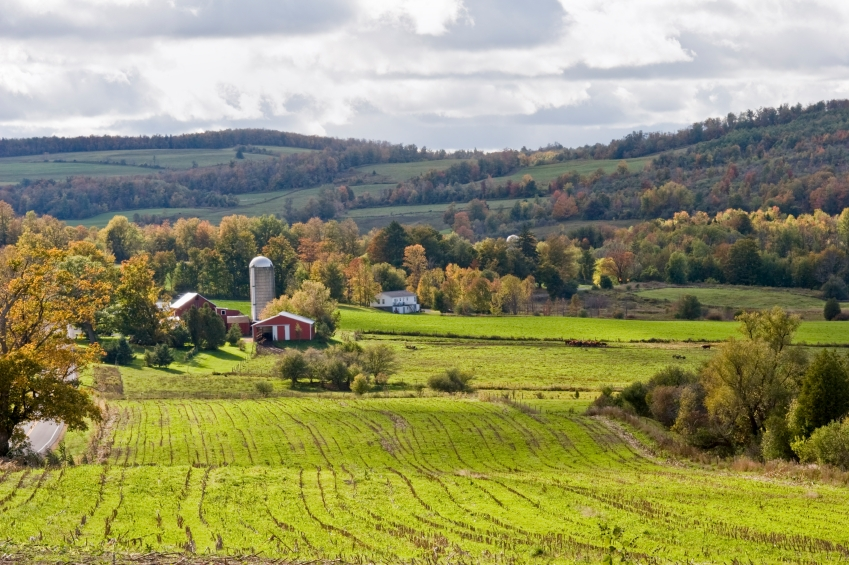
\includegraphics[width=1.5in]{farm}
%   \column{1.5in}
%   \textbf{P}artial \\
%   \textbf{E}quilibrium \\
%   \textbf{E}conomic \\
%   \textbf{L}and Use
%   \end{columns}
% \end{frame}

\begin{frame}
  \frametitle{Introduction}
  \framesubtitle{PEEL model}
  \begin{columns}[c]
    \column{2.0in}
    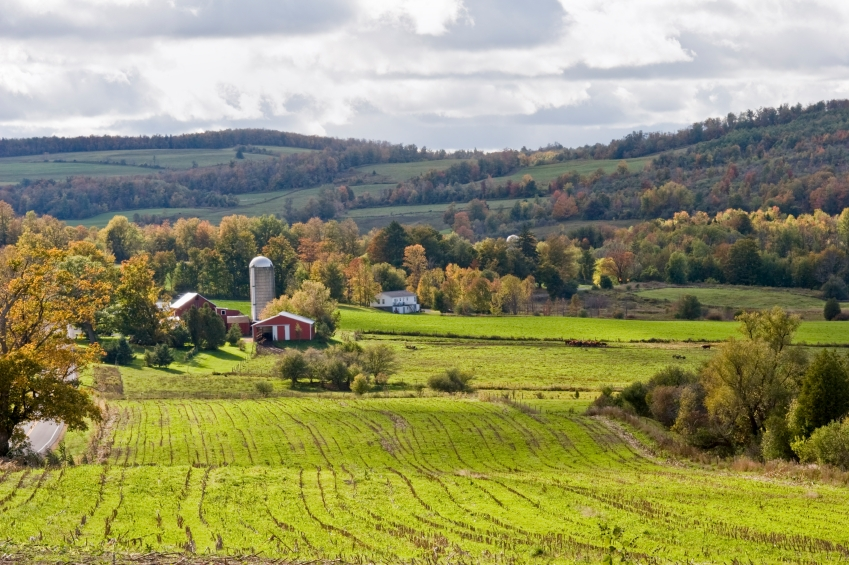
\includegraphics[width=2.0in]{farm} \\
    \vspace{0.25in}
    \textbf{P}artial \\
    \textbf{E}quilibrium \\
    \textbf{E}conomic \\
    \textbf{L}and Use
    \column{2.5in}
    For forecasting\dots
    \pause
    \begin{itemize}
    \item 
      Land use conversion to\slash from cropland
      \pause
    \item 
      Choice among locally viable crops for cultivation under profit maximization
    \end{itemize}
  \end{columns}
\end{frame}


\section{Objectives}

% \subsection{Data Set Synthesis}
% \begin{frame}{Data Set Synthesis}{Application}
% PEEL model will forecast\dots
% \begin{itemize}
%   \item 
%     \pause
%     Land conversion to\slash from cropland
%   \item 
%     \pause
%     Local blends of crops planted
%   \end{itemize}
% \end{frame}

\begin{frame}
  \frametitle{Objectives}
  \framesubtitle{Data Set Synthesis}
  Requirements
  \begin{itemize}
  \item 
    5 arc-minute resolution
    \pause
  \item 
    Sub-pixel analysis
    \pause
  \item 
    Global extent (eventually)
    \pause
  \item 
    Annual time series (eventually)
  \end{itemize}
\end{frame}


\begin{frame}
  \frametitle{Objectives}
  \framesubtitle{Reproducible Research}
  Advantages
  \begin{itemize}
  \item 
    Analysis runs like a program
    \pause
  \item 
    Final output is a publication-quality PDF
    \pause
  \item 
    Maps, charts, tables updated in place
    \pause
  \item 
    Source code and base data subject to review
  \end{itemize}
\end{frame}


\begin{frame}
  \frametitle{Objectives}
  \framesubtitle{Reproducible Research}
  Software Tools
  \begin{columns}[c]
    \column{1.0in}
    
\includegraphics[width=1.0in]{latex}
    \vspace{0.5in}
    
\includegraphics[width=0.75in]{r}
    \column{2.0in}  
    \begin{itemize}
    \item 
      \LaTeX \\ (typesetting)
      \pause
    \item 
      R \\ (analysis) 
      \pause
    \item 
      Sweave \\ (preprocessing)
      \pause
    \item 
      other R add-on packages \\
      ( raster, ggplot2)
    \end{itemize}
  \end{columns}
\end{frame}

\section{Data Sets}

% \begin{frame}
%   \frametitle{Data Sets}
%   \framesubtitle{MODIS Land Cover Type (MLCT)}
%   \begin{itemize}
%   \item Resolution: $\sim$500 m (15$''$)
% % try \second from mathabx if $''$ doesn't work
%   \item 3 layers
%     \begin{itemize}
%     \item Primary class
%     \item Secondary class
%     \item Confidence level
%     \end{itemize}
%   \item 17 classes simplified to 9
%   \item Mosaic contains 40--60\% crop
%   \item Annual time series 2001--2008
%   \end{itemize}
% \end{frame}

% \begin{frame}{Data Sets}{Detail of MLCT Primary Class}
%   \begin{center}
%     \includegraphics[height=2.75in]{fig_thumb_pri_reclass}
%   \end{center}
% \end{frame}


% \begin{frame}
%   \frametitle{Data Sets}
%   \framesubtitle{MODIS Land Cover Type (MLCT)}
%   \begin{columns}
%     \column{2.5in}
%     \includegraphics[width=2.5in]{fig_thumb_pri_reclass}
%     \column{2.5in}
%     \begin{itemize}
%       \pause
%     \item Resolution: $\sim$500 m (15$''$)
%       \pause
%     \item 17 classes simplified to 9
%       \pause
%     \item Mosaic contains 40--60\% crop
%       \pause
%     \item Annual time series 2001--2008
%     \item 3 layers
%       \begin{itemize}
%         \pause
%       \item Primary class
%       \end{itemize}
%     \end{itemize}
%   \end{columns}
% \end{frame}

\begin{frame}
  \frametitle{Data Sets}
  \framesubtitle{MODIS Land Cover Type (MLCT)}
  \begin{columns}
    \column{2.5in}
      \includegraphics<-6>[width=2.5in]{fig_thumb_pri_reclass}
      \includegraphics<7>[width=2.5in]{fig_thumb_sec_reclass}
      \includegraphics<8>[width=2.5in]{fig_thumb_pct}
    \column{2.5in}
    \begin{itemize}
    \item Resolution: $\sim$500 m (15$''$)
      \pause
    \item 17 classes simplified to 9
      \pause
    \item Mosaic contains 40--60\% crop
      \pause
    \item Annual time series 2001--2008
      \pause
    \item 3 layers
      \begin{itemize}
        \pause
      \item Primary class
        \pause
      \item Secondary class
        \pause
      \item Confidence level        
      \end{itemize}
    \end{itemize}
  \end{columns}
\end{frame}

% \begin{frame}
%   \frametitle{Data Sets}
%   \framesubtitle{MODIS Land Cover Type (MLCT)}
%   \begin{columns}
%     \column{2.5in}
%     \includegraphics[width=2.5in]{fig_thumb_sec_reclass}
%     \column[T]{2.5in}
%     Secondary class
%   \end{columns}
% \end{frame}

% \begin{frame}
%   \frametitle{Data Sets}
%   \framesubtitle{MODIS Land Cover Type (MLCT)}
%   \begin{columns}
%     \column{2.5in}
%     \includegraphics[width=2.5in]{fig_thumb_pct}
%     \column[T]{2.5in}
%     Confidence level
%   \end{columns}
% \end{frame}

% \begin{frame}
%   \frametitle{Data Sets}
%   \framesubtitle{National Land Cover Database (NLCD)}
%   \begin{itemize}
%     \item Resolution: $\sim$30 m (1.25$''$)
%     \item Single thematic layer
%     \item 29 classes simplified to 8
%     \item No mosaic class
%     \item 2001 only
%   \end{itemize}
% \end{frame}

% \begin{frame}
%   \frametitle{Data Sets}
%   \framesubtitle{Detail of NLCD}
%   \begin{center}
%     \includegraphics[height=2.75in]{fig_thumb_nlcd_reclass}    
%   \end{center}
% \end{frame}

\begin{frame}
  \frametitle{Data Sets}
  \framesubtitle{National Land Cover Database (NLCD)}
  \begin{columns}
    \column{2.5in}
    \includegraphics[width=2.5in]{fig_thumb_nlcd_reclass}    
    \column{2.5in}
    \begin{itemize}
      \pause
    \item Resolution: $\sim$30 m (1.25$''$)
      \pause
    \item Single thematic layer
      \pause
    \item 29 classes simplified to 8
      \pause
    \item No mosaic class
      \pause
    \item 2001 only
    \end{itemize}
  \end{columns}
\end{frame}

\begin{frame}
  \frametitle{Data Sets}
  \framesubtitle{Comparison of MLCT Primary and NLCD}
  \begin{columns}
    \column{2.5in}
    \includegraphics[width=2.5in]{fig_thumb_nlcd_reclass}    
    \column{2.5in}
    \includegraphics[width=2.5in]{fig_thumb_pri_reclass}    
  \end{columns}
\end{frame}

\begin{frame}
  \frametitle{Data Sets}
  \framesubtitle{Agland2000 (Ramankutty, et al.; 2008)}
  \begin{columns}
    \column{2.5in}
    \includegraphics[width=2.5in]{fig_thumb_agland}    
    \column{2.5in}
    \begin{itemize}
    \item Advantages
      \begin{itemize}
        \pause
      \item Census-based
        \pause
      \item 5$'$ resolution
        \pause
      \item Global extent
      \end{itemize}
      \pause
    \item Challenges
      \begin{itemize}
        \pause
      \item Different land mask
        \pause
      \item Be aware of circularity w\slash{}MLCT!
      \end{itemize}
    \end{itemize}
  \end{columns}
\end{frame}

% \begin{frame}
%   \frametitle{Data Sets}
%   \framesubtitle{175Crops2000 (Monfreda, et al.; 2008)}
%   \begin{itemize}
%   \item Advantages 
%     \begin{itemize}
%     \item Census-based
%     \item 5$'$ resolution
%     \item disaggregated by crop
%     \end{itemize}
%   \item Challenges
%     \begin{itemize}
%     \item Different land mask
%     \item Too many sub-classes
%     \end{itemize}
%   \end{itemize}
% \end{frame}


\section{Data Processing}
\label{sec:subpix}

\begin{frame}
  \frametitle{Data Processing}
  \framesubtitle{Sub-pixel Areas and Aggregation}
  \begin{center}
    \includegraphics<1>[height=2.75in]{fig_thumb_fracs}
    \includegraphics<2>[height=2.75in]{fig_thumb_agg}
  \end{center}
\end{frame}

% \begin{frame}
%   \frametitle{Data Processing}
%   \framesubtitle{Detail of MLCT Secondary Class in Facets}
%   \begin{center}
%     \includegraphics[height=2.75in]{fig_thumb_sec_facet}
%   \end{center}
% \end{frame}

% \begin{frame}
%   \frametitle{Data Processing}
%   \framesubtitle{Sub-pixel Areas and Aggregation}
%   \begin{center}
%     \includegraphics[height=2.75in]{fig_thumb_agg}
%   \end{center}
% \end{frame}

\begin{frame}
  \frametitle{Data Processing}
  \framesubtitle{Mosaic Decomposition}
  \begin{itemize}
  \item Mosaic land is 50\% crop land
    \pause
  \item Remainder is blend of forest, open, and shrub (by definition)
    \pause
  \item That blend is proportional to their presence elsewhere in the same 5$''$ grid cell (our assumption)
    \pause
  \item If none of those classes are represented we assume an equal blend of all three
  \end{itemize}
\end{frame}

\begin{frame}
  \frametitle{Data Processing}
  \framesubtitle{Mosaic Decomposition}
  \begin{center}
    \includegraphics<1>[width=2.5in]{fig_thumb_agg}
    \includegraphics<2>[width=2.5in]{fig_thumb_nomos}
  \end{center}
\end{frame}

\section{Comparison and Adjustment}
\label{sec:analysis}

\begin{frame}
  \frametitle{Comparison and Adjustment}
  \framesubtitle{Total Areas}
  \begin{center}
    \includegraphics[height=2.75in]{fig_areas}    
  \end{center}
\end{frame}

\begin{frame}[label=scatPlot1]
  \frametitle{Comparison and Adjustment}
  \framesubtitle{MLCT Crop vs. Agland2000, $A_{min}=1.0$}
  \begin{center}
    \includegraphics[height=2.75in]{fig_scatPlot1}    
  \end{center}
\end{frame}

\begin{frame}[label=scatPlot05]
  \frametitle{Comparison and Adjustment}
  \framesubtitle{MLCT Crop vs. Agland2000, $A_{min}=0.5$}
  \begin{center}
    \includegraphics[height=2.75in]{fig_scatPlot05}    
  \end{center}
\end{frame}

\begin{frame}
  \frametitle{Comparison and Adjustment}
  \framesubtitle{NLCD Offsets}
  \begin{center}
    \includegraphics[height=2.75in]{fig_offsets}    
  \end{center}
\end{frame}

\begin{frame}
  \frametitle{Comparison and Adjustment}
  \framesubtitle{Total Areas, Adjusted}
  \begin{center}
    \includegraphics[height=2.75in]{fig_areasAdj}    
  \end{center}
\end{frame}

\againframe{scatPlot1}

\againframe{scatPlot05}

\begin{frame}
  \frametitle{Comparison and Adjustment}
  \framesubtitle{MLCT Crop vs. Agland2000, $A_{min}=0.5$ plus NLCD offsets}
  \begin{center}
    \includegraphics[height=2.75in]{fig_scatPlotAdj}    
  \end{center}
\end{frame}

\section*{Summary}

\begin{frame}
  \frametitle{Summary}
  \framesubtitle{Next steps}
  \begin{itemize}
  \item Investigate spatial structure of 100\% crop cells in Agland2000
  \item Evaluate magnitude of cropland area classified by MLCT outside of Agland2000 land mask
  \item Re-allocate cells where Agland2000 crop fraction does not contradict NLCD offsets, i.e.:
    $A_{crop} \leq 1-A_{water}-A_{wetland}-A_{urban}$
  \item Disaggregate cropland into sub-categories (corn, soy, wheat, rice, other grains, etc.) using 175Crops2000 data set (Monfreda, et al.; 2008)
  \item Contribute to the underlying software!
  \end{itemize}
\end{frame}

\begin{frame}
  \frametitle{Summary}
  \begin{itemize}
  \item A rational framework for constructing a hybrid data set
  \item A basis for adding a time dimension by using the ensuing MLCT maps
  \item A repeatable mechanism for incorporating adjustments or evaluating alternatives
  \item A nicely formatted paper ready for publication somewhere!
  \end{itemize}
\end{frame}


%   % Keep the summary *very short*.
%   \begin{itemize}
%   \item
%     The \alert{first main message} of your talk in one or two lines.
%   \item
%     The \alert{second main message} of your talk in one or two lines.
%   \item
%     Perhaps a \alert{third message}, but not more than that.
%   \end{itemize}
  
%   % The following outlook is optional.
%   \vskip0pt plus.5fill
%   \begin{itemize}
%   \item
%     Outlook
%     \begin{itemize}
%     \item
%       Something you haven't solved.
%     \item
%       Something else you haven't solved.
%     \end{itemize}
%   \end{itemize}
% \end{frame}



% % All of the following is optional and typically not needed. 
% \appendix
% \section<presentation>*{\appendixname}
% \subsection<presentation>*{For Further Reading}

% \begin{frame}[allowframebreaks]
%   \frametitle<presentation>{For Further Reading}
    
%   \begin{thebibliography}{10}
    
%   \beamertemplatebookbibitems
%   % Start with overview books.

%   \bibitem{Author1990}
%     A.~Author.
%     \newblock {\em Handbook of Everything}.
%     \newblock Some Press, 1990.
 
    
%   \beamertemplatearticlebibitems
%   % Followed by interesting articles. Keep the list short. 

%   \bibitem{Someone2000}
%     S.~Someone.
%     \newblock On this and that.
%     \newblock {\em Journal of This and That}, 2(1):50--100,
%     2000.
%   \end{thebibliography}
% \end{frame}

\end{document}


